% !TeX root = ../thuthesis-example.tex

\chapter{绪论}


\section{研究背景及其意义}
\subsection{社团发现}\label{sec:community}
随着信息时代的到来,人类进入了网络化的世界。
绝大部分的网络均
存在一定的社团结构\cite{wang2012network}。
常见的社团结构有社交网络中的圈子、流行病网络中的疫区、自然界中的群落,
以及无线蜂窝网络中的小区等。
在网络科学中,社团结构是指
具有相同特征的节点集合, 属于同一社团的节点之间连接紧密,
而属于不同社团的节点之间连接稀疏。
而社团发现(也称为社团检测)作为网络科学研究的重点问题之一,是通过一定的方法寻找网络中特定的社团结构。
社团发现在社会工程、生物化学与计算机科学等领域均有着重要的应用。
比如在社会工程领域,
通过社团发现划分互联网社交媒体中的用户社群\cite{zalmout2013twitter},
用于舆情分析\cite{yang2018opinion}
或者推荐系统的设计\cite{cao2015recommendation};
在生物化学领域用于在蛋白质分子交互作用的网络中识别特定的功能模块 \cite{ayati2015mobas};
%研究中有助于发现特定的微观结构,
%在社会科学领域
在
计算机科学的分布式计算中需要将任务分配给不同的计算节点,
使得不同的任务之间有尽可能
小的耦合\cite{topcuoglu2002performance}。
如图 \ref{fig:distributed_computing} 所示,通过社团发现将
任务划分为不同的社团,可有效减少计算节点间数据传输的时间成本。

\begin{figure}[!ht]
    \centering
    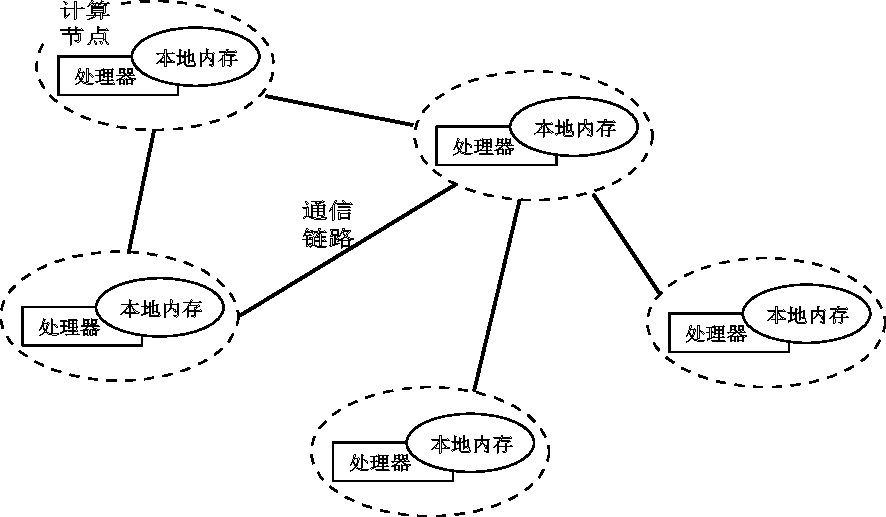
\includegraphics[width=0.6\textwidth]{background.pdf}
    \caption{分布式计算中的任务分配 (图源:\inlinecite{SITARAM2012351})}
    \label{fig:distributed_computing}
\end{figure}
%\footnotetext{图片来源于网络:\url{https://medium.com/@wisnu3121/how-distributed-computing-works-3dc0c8bdef10}}

% add a paragraph to praise the existing study of community detection algorithms

社团发现的实现离不开自动化算法的支撑,伴随着计算机科学的发展,
社团发现算法的发展主要经历了三个阶段。
在本世纪以前,社团发现主要是借用图划分或数据聚类的方法,
算法复杂度较高,仅适用于小规模的网络 \cite{fortunato2010community}。
得益于计算能力的提升,21世纪初十年代,以遗传算法为代表的随机优化策略被引入社团发现领域,
结合模块度(Modularity)的优化目标,涌现了大量的
社团发现算法。此外比较有代表性的方法还有利用贝叶斯方法进行模型的参数估计 \cite{jin2023survey}
等。
这些算法突破了网络规模的限制,可用于探测大规模复杂网络中的社团结构,并被逐步拓展到解决动态网络中的社团发现问题。
2010年以来,以深度学习为代表的人工智能技术开始应用到社团发现问题上来。
通过从图结构的数据中学习低维表示,该类方法在有节点辅助信息的场景中具有更大的灵活性
\cite{Su_2022}。

%而好的社团发现算法
%需要有特定的理论支撑,以便助其在各领域实现广泛应用。

尽管社团发现领域的算法研究不断取得突破,但目前对社团发现问题的
理论认识仍较为有限,成为了制约网络科学发展的瓶颈。
在算法设计层面上,由于缺少理论指导,算法设计往往以启发式的方式进行。
尽管这些算法在准确率上更胜一筹,但在实际问题中往往要进行超参优化与
多轮迭代,既消耗了大量的计算资源,同时检测效果也不一定能得到保障。
在算法评价层面上,由于在理论层面社团的概念缺少统一的定义,
难以公平合理地评估不同算法的优劣,从而给社团发现算法的选择造成了一定的困难。
在算法可靠性层面上,由于对算法的误差率缺少理论研究,
难以保证在标准数据集上表现良好的算法在新的问题上也能达到令人满意的效果
\cite{xiangxiang2021info}。

解决算法设计、算法评价与算法可靠性三大挑战应从新的视角入手。
考虑到网络中包含大量的节点信息和边的信息,
如果能合理度量并有效利用这些信息,则可以为社团发现理论研究和算法设计提供新的思路。
而信息论在这一方面体现出了巨大的潜力。

\subsection{信息论度量}
信息论的概念最早由香农提出,用以解决通信领域的问题 \cite{shannon1948mathematical}。
信息论的度量如熵、互信息等是概率分布的函数,
在对信源和信道的概率化建模的基础上,
用于度量信源编码和信道传输的理论极限。此外,信息论度量在统计推断
领域也有重要的应用,如假设检验问题中的误差指数、无偏估计误差的理论下界等。

在社团发现算法发展的第二个阶段,随着统计物理、生物信息学等领域的方法
纷纷被引入社团发现中,基于信息论的方法也不例外。
如图 \ref{fig:communication_community} 所示,
在社团发现中,
随机网络的生成与社团结构的划分可类比于通信过程的编码、传输和解码环节。
%目前,不同的学者对于具体建模过程的对应关系存在分歧,
%通过最大化互信息可实现
%但截止目前,笔者尚未找到这方面系统性的综述文章。
%以下是笔者不揣冒昧,试着对这一研究领域进行阶段性总结。


\begin{figure}[!ht]
    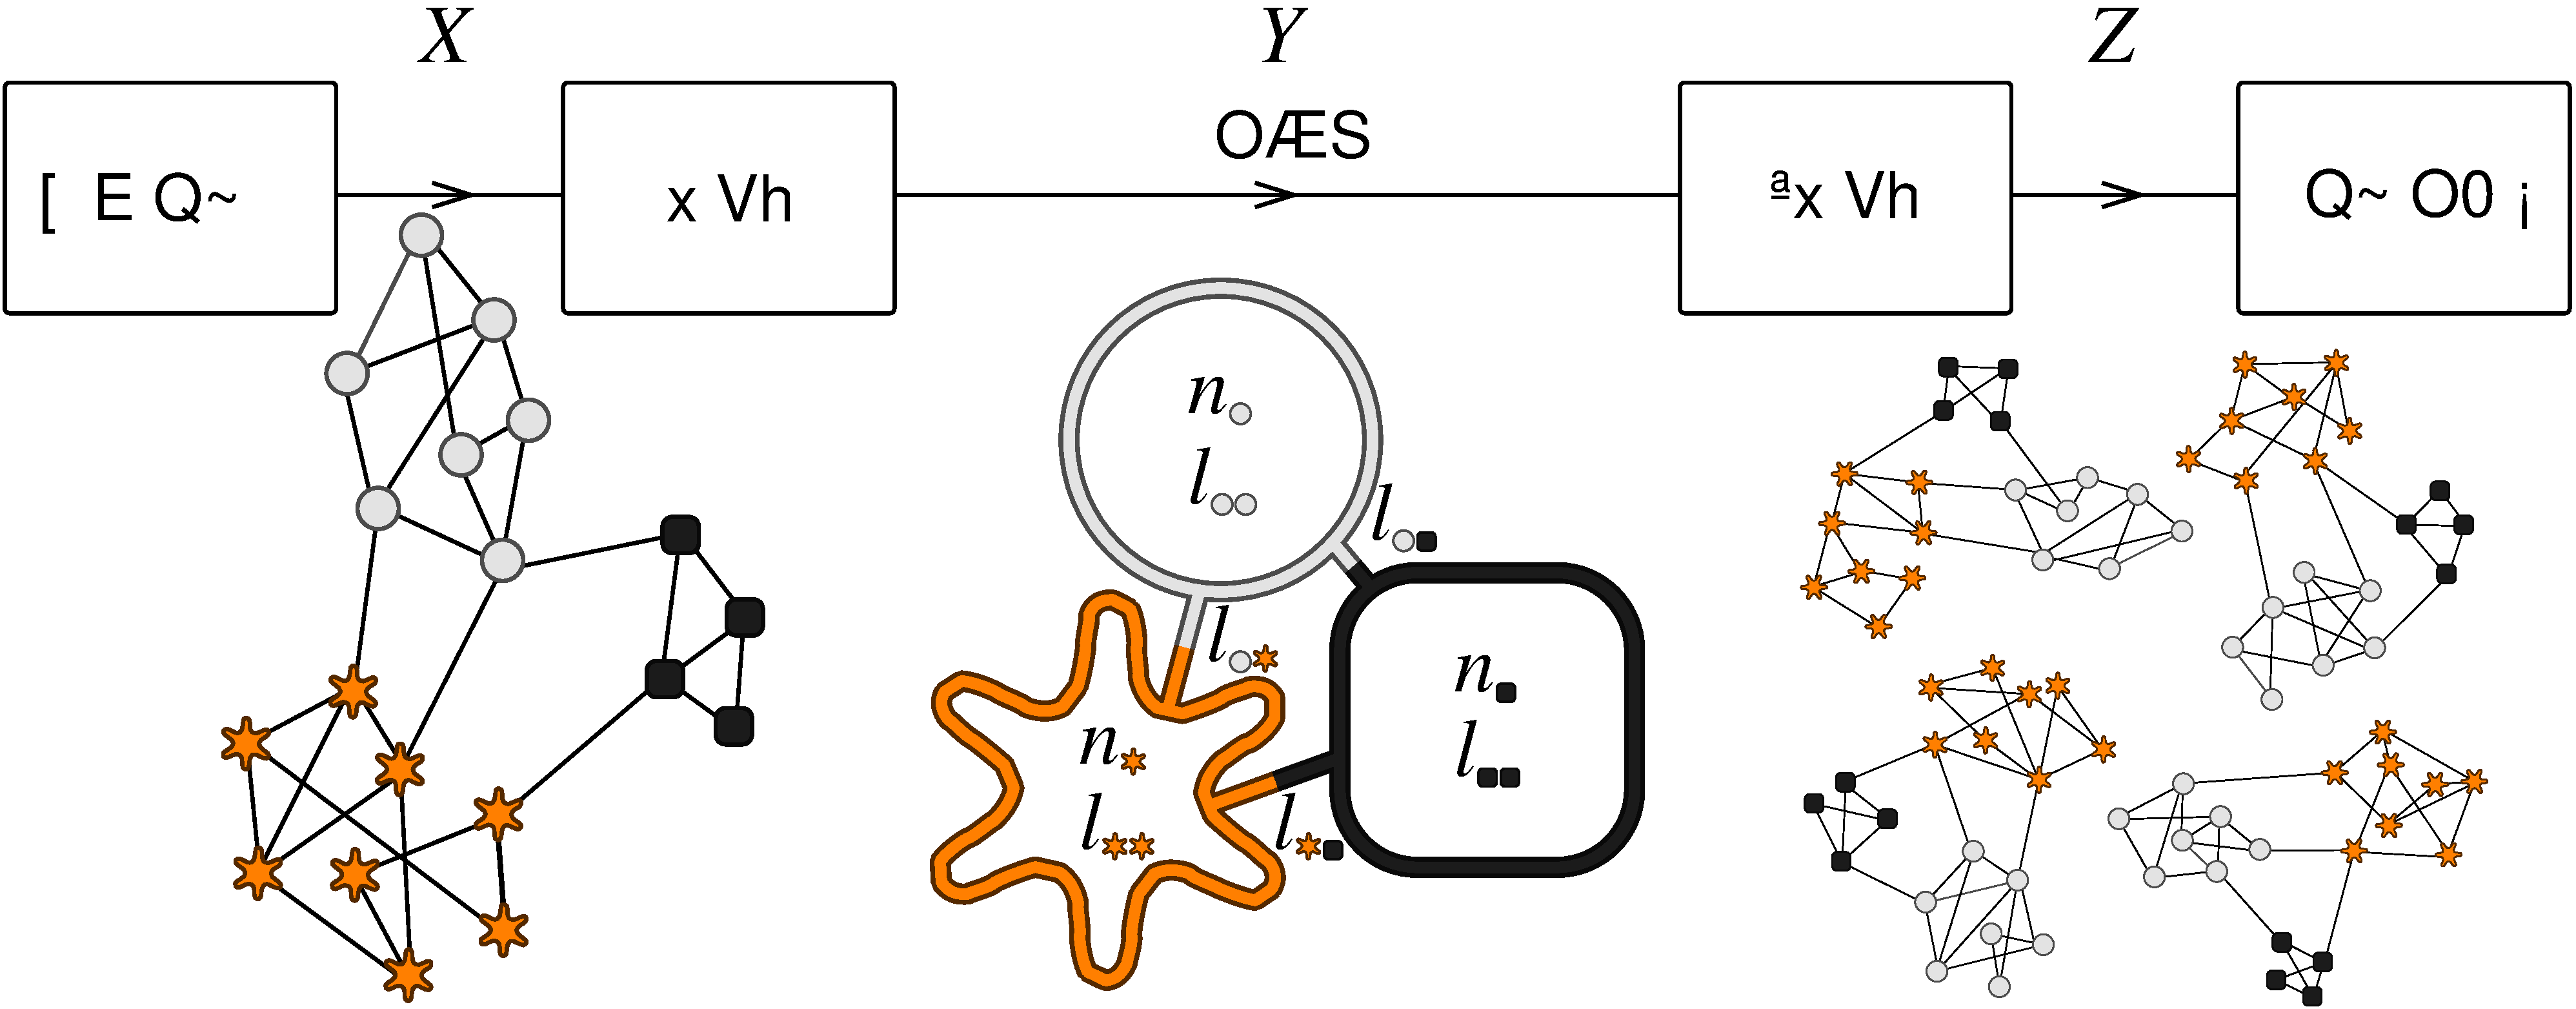
\includegraphics[width=\textwidth]{Rosvall07.pdf}
    \caption{将社团发现建模为通信过程的基本框架(图源:\inlinecite{rosvall2008mcl})}
    \label{fig:communication_community}
\end{figure}

在通信领域的问题研究中,信息论度量的成功应用有赖于可设计的概率模型,
而在实际的网络中则缺少这种概率分布的先验知识,
这给信息论度量在社团发现问题上的应用
造成了一定的困难。
而目前克服这一困难的方法主要分为以下两大类:

第一类方法首先把信息论度量应用在数据聚类问题上,
通过普适信息论的方法克服数据分布未知的困难\cite{raman20219}。
这里的普适性是指对数据的统计特征只做一般性假设而没有精确的先验知识。
由于数据聚类问题和社团发现问题可相互转化,社团发现算法性能评价指标与聚类评价指标
相互通用,从而基于普适信息论的数据聚类方法也可用于设计社团发现算法。

另一类方法是人为地引入随机性,一种常用的引入随机性的方法是使用随机图对数据进行建模。
随机图模型是对复杂网络的概率化建模,可模拟复杂网络的小世界、无尺度等特性。
对随机图模型的研究可类比信道编码领域编码误差的研究思路 \cite{abbe2015community}。
通过将随机图建模成有噪声的信道,可研究其最优恢复误差
以及如何设计多项式时间的算法以达到最优。
%对于随机图,可利用信息论度量研究带有社团结构的随机图的理论性质。
%本部分的研究主要类比了信道编码领域算法误差的研究思路。在信道编码中,通常研究给定信道时传输效率的理论极限,
%而在社团发现的研究中,则是给定输入的随机图模型,研究发现算法的理论极限。在理论极限的基础上,同样类似信道编码
%领域的研究,在社团发现领域,基于谱分解等方法社团发现算法理论极限的可达性已有相关研究,
另一方面,若不将网络看作由随机图模型生成,随机性仍可通过其他方式引入。
比如在基于最大化互信息的方法中,采用条件分布是均匀分布的假设
%社团描述量与随机网络的
\cite{rosvall2007information}。在社团数量未知的情况下,
可利用最小描述长度原理进行
社团发现\cite{chakrabarti2004autopart,rosvall2007information}。
再如,有学者提出通过优化图上的随机游走过程产生的序列码长进行社团发现的方法,
其中的概率质量函数利用随机游走的频率进行估计\cite{rosvall2008mcl}。
该研究也为利用社团发现的方法
解决图上的信息压缩问题提供了思路\cite{abbe17sideinfo}。
%结合对概念生成模型进行参数估计的方法,进行描述
%虽然在本世纪初信息论度量开始被用于与网络科学中社团发现问题相关的研究,
%但其面临着一个
%。

基于信息论的社团发现算法相比于经典的基于模块度优化的算法有着诸多的优势。
Rosvall等\cite{rosvall2007information} 指出模块度优化在各社团大小或度相差较大时
效果受限,而基于编码理论的方法可克服这一不足。此外,Abbe等\cite{abbe2015community,hajek2016achieving} 
使用信息论度量的方法分析了社团大小不一致的情形下算法的误差衰减情况,
并设计了可实现精确恢复的算法,而使用基于模块度优化的算法则难以实现
精确恢复的目标。

信息论度量主要在理论建模和算法设计层面有应用价值。
在理论建模层面上,信息论度量有助于节约计算资源。
通过优化能量函数进行社团发现的方法对于某些超参数值检测准确率低,
基于信息论度量的研究可以找出这些参数值的范围,从而在实际计算中
提升超参优化的效率,节约计算资源\cite{ye2020exact}。
其次,信息论度量能够保证社团发现算法的准确度。
比如在针对随机块模型(Stochastic block model)恢复误差的理论极限研究中,可以提前知道能否完全恢复其社团结构,
从而选用恰当的算法实现这一目的,保证恢复效果\cite{abbe2015community}。
在算法设计层面上,信息论度量可直接用于社团发现算法性能评价,
比如归一化的互信息(NMI)\cite{Danon_2005}、变分信息(VI) \cite{2007Comparing}等。
此外,信息论度量也可以指导设计能够达到最优误差率的算法,比如
有学者提出一种带惩罚因子的似然估计方法来达到通过信息论度量表示的
最优误差率\cite{zhang2016}。最后,基于普适信息论的数据聚类方法
也可直接用于社团发现算法的设计\cite{gokcay2002clustering, chan2017pin, app12094203}。

尽管信息论度量在社团发现领域的应用取得了一定的成功,但也存在
着一些不足之处。
一方面,
%针对基于信息论度量设计的社团发现方法,
%比如最优压缩率
%等方法,
由于实际含有社团结构的网络形态多种多样,
社团发现方法的效果仍需要通过大量实验来检验。
而从实验结果来看,无论是在算法复杂度还是准确率方面,
该类方法同应用最先进技术的启发式社团发现算法
相比还有一定的差距。另一方面,
在随机图的理论建模研究中,通常考虑图的规模趋向于无穷大,
该假设可能与实际网络不符,从而导致理论结果的应用价值也受到一定的限制。

\section{问题引出}
我们在上一节指出,使用信息论度量研究社团发现问题
主要有应用普适信息论和基于随机图两种思路。而社团发现有多个细分领域,
如重叠社团、动态网络、层次结构等。
我们沿着这两种思路,
从社团发现诸多细分领域中选取了社团层次发现、随机块模型和辅助信息三个细分领域深入开展研究。
%,
%可以有效地分析随机块模型及其变体的
%精确恢复条件和最优误差率等理论性质。

%但信息度量的基本概念“熵”则源自
%统计物理中的“熵”。无独有偶,在社团发现算法研究的第二个阶段统计物理家也开始对这一
%问题感兴趣,并将一些概念引入社团发现的算法。

%由于,对社团发现问题的概率模型的理论
%极限和部分经典算法的信息学含义缺少足够的认识,
%为解决该问题,需要对社团发现的理论模型开展深入研究。


首先,考虑到在某些实际问题中不同的社团之间具有包含关系,从而构成一定的层次结构。
比如一个年级分为不同的班级社团,每个班级社团包含若干学生节点。
再如从现存的物种之间
可以构造出层次树的结构,用来表示物种进化的历程。
普通的社团发现算法只能将网络划分为若干没有包含关系的社团,
无法适应社团层次结构划分的需要。因此,基于信息论的指导,
研究新的层次发现算法对解决特定应用场景下的社团发现问题
具有重要的实用价值。

其次,在对复杂网络进行建模时,随机块模型常用于生成有社团结构的网络,
为比较不同社团发现算法提供了标准化人工生成数据集。
此外,通过结合随机块模型的参数估计和选择等知识,
大量社团发现算法得以涌现。
但这些算法缺少对误差的理论分析,
对于大规模的随机块模型,无法预知其误差如何,
因而限制了其使用场景。
%此外,从理论层面研究随机块模型下算法的误差可以
%指导算法的设计。
目前的研究
针对随机块模型给出了若干具有理论保证的算法,通过对这些算法的优化目标做出近似和调整,
可以适用于实际的社团发现问题。
%随机块模型的研究
%还可以用于解决和社团发现密切相关的问题,比如根据若干次民意调查的结果预测选民的政治倾向等。

另外,在分析具有图结构的数据时,
通常每个节点会有一些辅助的信息可供使用,
如全部节点的特征属性或部分节点的标签属性等。
带有辅助信息的网络具有广泛的应用场景,比如在社交网络中利用
用户间的交互关系和每一用户自身的属性对用户群体进行划分。在生物信息学中利用
基因本身的信息和不同基因之间的互信息对基因进行聚类 \cite{4359897}等。
如何利用这些节点的观测值提高
社团发现算法的准确率也是近年来研究的一个热点。
已经涌现了大量的算法可以同时利用节点和边的信息进行社团发现,但在这方面缺少
针对误差率的理论分析。除算法设计外,这方面的理论分析工作也具有重要意义,
比如可以指导特征数量的选取,
以提高数据使用效率,降低计算成本等。



社团发现理论与算法的研究是一个涉及信息论、图论、概率论、统计物理和计算机科学等多学科交叉融合的领域。
信息论度量在社团发现问题上的成功应用,也离不开其他学科知识的帮助。通过融合多学科
领域的知识,社团发现的研究呈现出百花齐放的特点。
该特点在国内外已有研究方面体现得尤其明显,下面结合本文研究的三个主要问题
对国内外相关文献进行梳理。

\section{国内外研究动态}

社团发现领域的研究可大致划分为理论研究、算法设计与分析以及应用研究三个层面
\cite{ZJSH201102017}。结合本文的研究范畴,下面我们对理论研究和算法设计层面的已有工作
进行简要介绍。

\newglossaryentry{cbm}{name=审查块模型, description={Censored block model}}

在理论层面主要是利用数学工具研究网络规模趋向于无穷大时社团发现的相变现象
\cite{lenka2016physics}、
算法的最优误差率与特定算法的误差率等内容。通常需要
采用随机图对网络进行建模,常用的随机图模型有随机块模型
\cite{holland1983stochastic},
审查块模型(Censored block model) \cite{hajek2015censored}等。
针对这些随机图模型,可以设计出有理论保证的社团发现算法。%[其他范式的理论研究]
%涉及该部分研究的多为概率统计学、统计物理和信息论等学科的文献。
%有理论保证是指这一类算法针对随机块模型可以实现节点标签的精确恢复。

%通过配置随机块模型的参数,可以生成具有不同结构的随机图。反之也可以通过给定的图估计随机块模型的参数\cite{RJXB201609005}。
%除此之外,在随机块模型参数已知的情况下,

相比于理论研究关注于算法机理解释与极限情形下的误差,
在算法设计层面的研究则更关注算法复杂度以及算法在不同人工生成与实际网络上的效果。
在 \ref{sec:community} 节已介绍了社团发现算法三个阶段的发展历程,
目前理论层面的工作聚焦于研究第二阶段涌现出的算法,
我们这里也对这类算法进行简要介绍。
此类算法一般是近似求解一个整数优化问题,
该类问题通常没有多项式时间的解法,
但可以通过启发式方法或松弛为一个数值优化的问题近似求解。
社团发现的优化目标主要有
模块度的最大值 \cite{newman2006modularity},汉密尔顿能量的最小值
\cite{reichardt2004potts} 等。另外,有学者基于信息论度量提出了
最小描述长度\cite{rosvall2007information}和信息瓶颈\cite{ziv2005bottleneck}等优化指标。
启发式求解算法主要有
去除图中的边\cite{girvan2002community}、
聚合图中的点 \cite{clauset2004finding}、
模拟退火\cite{massen2005annealing}、
标签传播\cite{raghavan2007near}、
元胞自动机\cite{chen2008automata}
和遗传算法 \cite{pizzuti2008ga, zhu2009genetic}等。
利用数值计算求解的算法主要有谱分解\cite{coja-oghlan_2010}和半正定规划\cite{chen2012sdp}等。
%此外,在算法设计层面也有大量的相关研究在中文学术圈发表。
%应用层面的研究主要集中在生物网络和社交网络方面,通常需要和特征提取等工程步骤结合起来才能实现一次比较有意义的数据挖掘工作。

如同前一节所介绍的, 本课题主要包含层次化发现算法、随机块模型及有辅助信息的社团发现三个方面的研究内容。
下面将分别从这三个方面进一步阐述国内外研究的动态。
\subsection{层次化发现算法}
考虑到社团发现问题的研究和数据聚类问题有共通之处,
很多针对数据的层次聚类算法可以直接用到社团发现领域中来,
%即都是将数据划分出一定的层次结构。不同之处在于数据的形式不同,
%聚类中考虑的是每个数据都有一个特征向量,而社团发现是针对图的数据结构。这两类结构之间是可以相互转换的,比如通过
%k近邻的方法可以从数据特征构造表征数据间相似程度的图。反之,通过特征嵌入 (feature embedding) 的技术由图可以
%获取每个节点的数据特征 \cite{hamilton2017representation}。通过这样的相互转换,聚类算法和社团发现算法可以通用。但由于这种转换会损失掉一部分原始信息
%并且具有一定的计算复杂度,通常意义上的聚类算法直接针对向量型的数据进行处理而社团发现是针对图进行处理。通过使用图的结构对网络
%进行数学建模,社团即是图的子图。
%但在社团的定义这一问题上仍没有定论,通常要在所研究的具体问题背景下合理定义。比如在
%研究网络社团中,有学者提出了一种新的网络社团的定义方式,方便进行社团的层次化发现
%\cite{alphabetaclustering2019}。
%最早的层次化发现算法是系统聚类法 \cite{slink},
%即根据欧式度量每次聚合两个节点形成聚类树。
%近年来基于各领域学科知识提出的层次聚类算法,
或者启发社团层次化发现算法的设计。
%比如
%贝叶斯层次聚类方法 \cite{heller2005bhc}、
%基于图论和离散数学的方法 \cite{dasgupta2016cost}。
%这些方法在模型复杂性,效率和准确性方面有着不同的权衡。
例如,基于贝叶斯层次聚类\cite{heller2005bhc},
有学者提出相应的贝叶斯社团发现算法\cite{blundell2011discovering, blundell2013bhcd},
在给定的概率模型下
可以产生非二叉结构的层次树。
%贝叶斯聚类的方法考虑了数据的分布,不能直接用于社团发现的场景。有学者将其进行改造,提出了
%贝叶斯社团发现的算法,在某些数据集上有较好的表现。
%贝叶斯模型总体说来有许多超参数需要调整,其层次化发现结果可能因其固有的随机性而有很大差异。
%因此,在实际应用中,不适合使用基于贝叶斯的模型来解决具有稳定需求的问题。 
再如,
%除了上面提到的分层发现方法外,
有学者利用信息论度量代替传统层次聚类中的指标
\cite{gokcay2002clustering,aghagolzadeh2007hierarchical,chan2016ic},
其中,Chan等\cite{chan2016ic}提出的多变量互信息的指标
%这些数据主要是根据经验得出的,可能无法反映出数据真实的概率模型。
%在过去的文献中,使用了其他某种信息理论量度 \cite{gokcay2002clustering} 或互信息\cite{mim}
%来做为聚合的标准。
%这些现有研究存在一些缺点。首先,信息度量是使用 Parzen 窗口根据数据进行估计的,该窗口是一种高斯混合模型。对于这种参数化方法,如果数据真实的分布与假设相距甚远,则结果会很不准确。
%其次,只有贪心算法才能逼近基于信息论的损失函数的最小值。 
%直到有学者提出群集中的多元互信息度量标准后,在这一方面才有所突破 \cite{chan2016ic}。 
可应用到社团发现领域\cite{chan2017pin}。
%该多变量互信息的度量可以处理对随机变量进行聚类的问题,在两两独立的网络模型 \cite{chan2017pin}
%中其数学结构与最小平均损失一致  \cite{mac}。最小平均损失,也叫图强度 \cite{cunningham1985optimal},
%是在不给定划分数的情况下求解
%平均最小割问题。与最小割是NP难不同的是,最小平均损失可以在多项式时间内求解。
%第一个算法由 Narayanan 提出,利用了主分格序列这样一种结构 \cite{narayanan}。
%后面有人通过参数化最大流的方式加以改进 \cite{pic}。

除了利用数据聚类的算法外,
也有大量的工作直接针对社团发现问题设计层次化发现算法。
这些算法可大致分为三类\cite{li2022hierarchical}:
直接估计层次树的结构\cite{arenas2006synchronization, blundell2013bhcd}、
自顶向上的聚合方法\cite{clauset2004finding}
和自顶向下的分裂方法\cite{girvan2002community, dasgupta2016cost}。
\highlight{聚合方法和分裂方法得到的层次结构一般并不相同,
从而限制了社团层次化问题的理论分析建模}\cite{chan2020agglomerative}
\highlight{。除此之外,现有的社团层次化发现方法往往针对特定的应用场景且侧重于算法设计层面的研究,对社团层次化结构的理论性质和最优划分%
缺乏深入的了解,从而导致所设计的算法通用性差,且对求解得到的层次化结构解释性较差。
为克服这一困难,我们从多变量互信息度量的角度出发,建立社团层次化发现的数学模型,
在理论和算法两个层面对层次化发现问题进行深入分析。}

%异常值检测问题 \cite{grubbs1969procedures} 和聚类分析有着密切的联系,
\subsection{随机块模型的精确恢复问题}
随机块模型是一种生成图模型,常作为度量不同社团发现算法的基准数据集,
在机场客流分析\cite{zhao2016rfla}、信息检索的主题模型\cite{Gerlach_2018}等领域也有广泛应用。
%它的另一个名称是 种植 k-分区模型,其中 $k$ 是社团的数量 。
随机块模型的生成方法是先给定 $n$ 个节点,再根据节点所属的类别随机地生成边。
同类节点之间有边相连的概率  $p$ 大于
不同类节点之间有边相连的概率 $q$ \cite{abbe2017community}。

在使用信息论的知识对随机块模型开展理论研究的现有工作中,
衡量算法的恢复性能通常使用错误率的方式。
这些工作考虑了在何种条件下,随着图中节点数量 $n$ 趋向于无穷,
错误率趋向于零。
错误率有几种不同的定义,
与之相对应,通过算法恢复原随机块模型社团结构也有多种目标
:精确恢复 (Exact recovery) 、几乎完全恢复、弱恢复和部分恢复
\cite{abbe2017community}。
其中,精确恢复是考虑全部节点不出错的情况。
在信息论的编码理论中,由于可靠传输的要求,往往使用精确恢复的标准衡量算法的好坏。
而在高可靠性的场景下,精确恢复的目标在社团发现领域也有实用价值。
因此,本部分借鉴信道编码理论中的研究方法,选取精确恢复作为重点研究的社团结构恢复要求。

%在弱恢复的研究中,通常是考虑 $p, q$ 在 $\frac{1}{n}$ 这一数量级,因为对于更稀疏的图,无法实现弱恢复的目标。
%对于两类的随机块模型并且 $p=\frac{a}{n}, q = \frac{b}{n}$。2014年前后证明了弱恢复的充要条件是 $(a-b)^2 > 2(a+b)$
%\cite{mossel2015reconstruction, mossel2018proof}。

在精确恢复的研究中,通常是考虑 $p, q$ 在 $\frac{\log n}{n}$ 这一数量级,
即 $p,q=\upTheta \left(\frac{\log n}{n} \right)$。
因为对于更稀疏的图,即$p, q=o\left(\frac{\log n}{n} \right)$,
无法实现精确恢复的目标。
而对于更稠密的图,即$p,q=\omega\left(\frac{\log n}{n} \right)$,
精确恢复的误差总是衰减到零的。
对于有两个社团的随机块模型,
在参数取值为 $p=\frac{a \log n}{n}, q = \frac{b \log n }{n}$
的条件下,精确恢复的充要条件是
$\sqrt{a} - \sqrt{b} > \sqrt{2}$ \cite{abbe2015exact, mossel2016}。
这个结果随后推广到了有 $k$ 个社团以及更一般的随机块模型中\cite{abbe2015community}。

\newglossaryentry{ising}{name=伊辛模型, description={Ising model}}
在关于随机块模型的变体研究中,有多种拓展的思路可以将$\sqrt{a} - \sqrt{b} > \sqrt{2}$
这一充要条件作为特例导出,
如 互测量 \cite{chen2016information}、 最小最大速率 \cite{zhang2016} 等。
在这其中,一类结合了伊辛模型 (Ising model)的工作融合了统计物理中的相变理论与信息论中的误差率\cite{ye2020exact},
为随机块模型精确恢复问题的研究开辟了新的思路。
在其关于样本复杂度研究中,$\sqrt{a} - \sqrt{b} > \sqrt{2}$是一个必要的前提。
%因此该复合模型可看作随机块模型的一个拓展。


%关于 随机块 模型算法错误率的一个误差上界在推导精确恢复的充分条件时给出 \cite{abbe2015exact},
%但有提升空间。
%相比之下,弱恢复的最优误差率渐近表达式可以写成两个伯努利变量的雷尼散度的形式 \cite{zhang2016}。

在算法层面,除了常用于理论证明的最大似然算法可实现精确恢复外,
基于半正定规划\cite{hajek2016achieving,amini2018semidefinite}、
谱分解\cite{Yun2014} 的方法也被证明具有实现精确恢复的能力。
而对于这些算法之间关系的探讨也有相关的研究结果。
%基于最大似然算法的改进算法也可用于恢复随机块模型的结构,并且在真实数据集上有良好的效果
%\cite{karrer2011stochastic}。
%基于此,
比如关于最大似然算法和最大模块度算法在度修正的随机块模型上的等价性已有学者进行了研究 \cite{newman2016equivalence}。
%最大模块度算法的优化目标是 NP 难的,最早使用贪心法近似求解 \cite{clauset2004finding},后来有学者使用模拟退火的方法近似求解 \cite{he2016fast}。
此外,还有学者提出了非凸优化的方法检测随机块模型的社团结构,
并证明了该方法具有精确恢复的能力\cite{wang2021non}。
%模拟退火的方法和 梅特罗波利斯 (Metropolis) 采样算法原理一样,只是表述不同,后者常用于 伊辛 模型的采样 \cite{metropolis1953equation},
%而前者是求解黑盒优化问题的启发式算法之一。

%在算法设计层面,利用 对称的 随机块 的结构,基于 ADMM 的迭代策略,有学者提出了 SDP-1的算法 \cite{amini2018semidefinite}。

\highlight{针对随机块模型,现有工作设计的达到精确恢复条件的算法较为复杂,
即使是基于谱分解的方法也要增加必要的前后处理步骤,且在精确条件不满足时大多数工作未给出
算法误差。为克服这一不足,我们提出一种基于玻茨模型(Potts model)的社团检测方法,
给出了不同参数条件下的恢复误差。
}


\subsection{有辅助信息的随机块模型}
\newglossaryentry{side_info}{name=辅助信息, description={Side information}}
通过添加辅助信息 (Side information),社团发现能达到更高的准确率。
通常的辅助信息是指节点属性信息\cite{he2019attribute},
其在理论分析中可以采用多种形式建模,
比如已知部分节点的标签、已知被噪声污染的全部节点的标签、
以及已知每个节点附带的一些观测值等\cite{saad2018community}。
使用信息论方法的现有研究
通常将网络建模成由随机块模型生成,而把仅用辅助信息进行各节点状态估计视为若干独立的假设检验问题\cite{ahn2023testing}。
辅助信息的引入可以提高社团发现的精度,从另一个角度看网络结构也可以提高群体检验的精度。
%这一部分的研究工作可以应用在社交网络分析中,比如利用用户间的交互关系与
%每一用户自身的属性对用户群体进行划分。

类似于上一小节没有辅助信息的场景,我们根据社团发现的恢复目标对现有工作进行分类。
围绕着精确恢复问题,有辅助信息的随机块模型研究内容通常包括精确恢复条件和实现精确恢复的算法等。
%已知正常标签的节点、全部节点的标签通过一个二元对称信道两种情形,
有学者考虑了多种类型的辅助信息,并在随机块模型精确恢复条件的基础上
给出了拓展模型精确恢复的充要条件\cite{saad2018community, esmaeili2019community}。
% one result comes from 2021 ISIT submitted paper
而对于辅助信息是每个节点附带的观测值的场景,有学者在
研究图上的数据压缩问题时顺带给出了一个精确恢复的充要条件 \cite{abbe17sideinfo}。

%对称分布的一般假设检测问题的特例 \cite{gao2018community}。
在算法层面,利用半正定规划算法检测带有部分节点标签的 随机块模型,
可实现精确恢复 \cite{esmaeili2019exact},
通过引入更多的优化参数,基于半正定规划的算法可用于一般的属性网络社团发现问题
\cite{tang2023semidefinite}。

%是最大似然算法好的近似 。

在有辅助信息的场景下,围绕着其他类型的恢复问题,比如几乎完全恢复,也有大量相关的研究\cite{kanade2016global, deshpande2018contextual}。
\highlight{而本部分的研究重点是半正定规划的精确恢复能力。现有使用半正定规划方法的目标函数是
用辅助信息构造的相似度矩阵与图的邻接矩阵进行加权得到的,在有属性分布的先验信息的情况下求解该优化问题
不能取得最优的检测效果。而我们从似然函数出发得到带有辅助信息的优化目标,通过半正定松弛的技巧
进行求解,在理论分析层面上可实现精确恢复。}

\section{研究方法与论文结构安排}
如前所述,本课题在已有的信息论方法研究社团发现的基础上,提取出了
普适信息论和基于随机图建模两种主要手段,并应用它们
深化社团发现领域的现有研究。具体来说,我们使用多变量互信息的度量研究社团
层次发现的性质、算法效率的提升等内容;而在随机图建模方面,则综合运用
速率函数(Rate function)、雷尼
%\footnote{北京大学出版社出版的《数学对话录》对于原作者使用雷尼的译名。}
散度(Rényi divergence)等
多种信息论度量对社团发现算法的理论极限进行刻画,
并借此开发新的高效算法。论文的结构安排如下:

% \subsection{层次化发现算法}
首先,在第 \ref{chp:knowledge} 章,我们对社团发现问题进行数学建模,
并简单介绍了本文用到的各种信息论度量及其他研究工具。

在第 \ref{chap:info_clustering} 章中,我们从普适信息论的视角出发,仅对随机变量的分布做一般
性假设,利用信息几何的知识探索多变量互信息在社团发现中的应用。
由于现有的多变量互信息计算方法复杂度过高,限制了
其在一般规模网络上进行层次结构发现。
在理论研究的基础上,我们有针对性地提出了高效算法降低其复杂度。
另外,我们考虑到基于多变量互信息的社团层次发现算法尚未有具体应用案例,
在本文中也给出了若干应用场景,弥补了这方面的不足。

% \subsection{随机块模型的精确恢复问题}
在第 \ref{chap:sibm} 章中,我们基于前一部分的研究中涉及的图划分的概念,
利用划分定义能量函数,进而构造图上的 玻茨模型,
并利用玻茨模型研究随机块模型的精确恢复问题。
这一部分的研究起到承上启下的作用,一方面,
它突破了前一部分普适信息论方法中
实际数据不满足假设条件与计算复杂度较高的局限性,
开始基于随机图的概率模型
对社团发现算法的理论极限进行定量刻画;
另一方面,它发展的理论研究工具,如速率函数等,
可以应用到后续的有辅助信息的随机块模型的研究中。
% \subsection{有辅助信息的随机块模型}

在前一章的研究基础上,第 \ref{chap:sbmsi} 章考虑了有辅助信息的随机块模型,
并通过错误概率的形式定量地刻画了辅助信息
对随机块模型精确恢复的贡献。
此外,本部分的另一个研究重点是证明
有辅助信息的随机块模型的精确恢复可由半正定规划算法实现。
在此基础上,我们设计了
求解半正定规划问题的高效迭代格式。

最后,第 \ref{chp:summary} 章对前几章的工作进行了总结,在此基础上对其中用到的分析技术给出了若干
评注。此外,我们还对基于信息论方法的社团发现未来研究方向进行了展望。